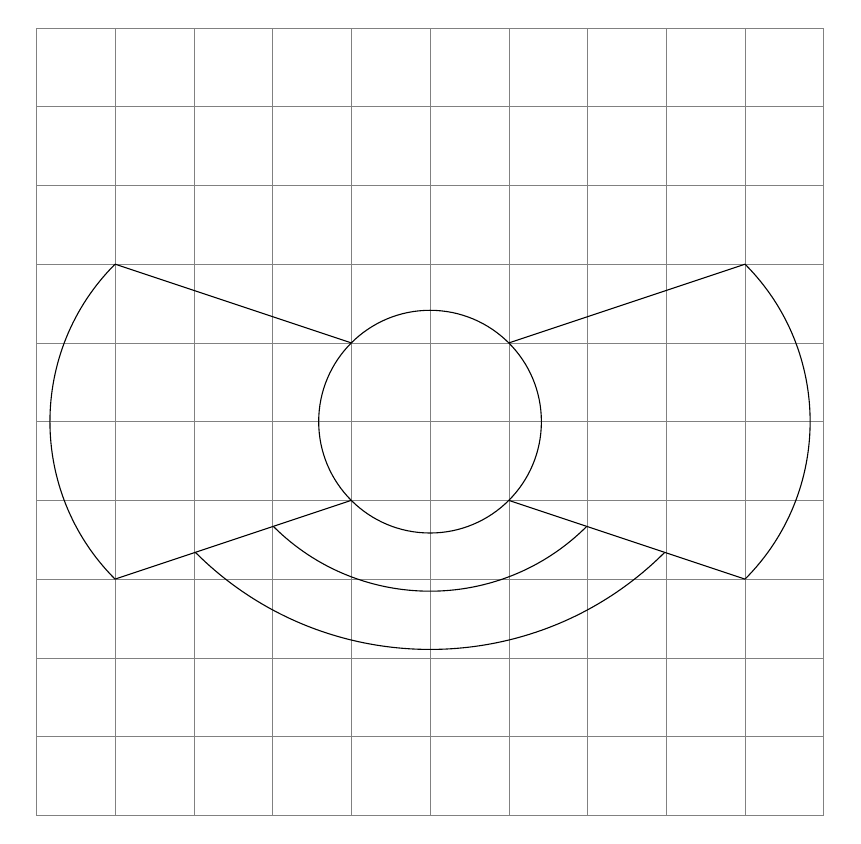
\begin{tikzpicture}
    \draw[help lines] (-5,-5) grid (5,5);
    
    \draw (0,0) circle [radius=1.41421356237];

    \draw (1,1) -- (4,2); 
    \draw (1,-1) -- (4,-2) node [pos=0.33, auto=left] (a) {} node [pos=0.66, auto=left] (c) {}; 
    \draw[out=45, in=135, relative] (4,2) to (4,-2); 

    \draw (-1,1) -- (-4,2);
    \draw (-1,-1) -- (-4,-2) node [pos=0.33, auto=right] (b) {} node [pos=0.66, auto=right] (d) {};
    \draw[out=-45, in=-135, relative] (-4,2) to (-4,-2); 

    % \draw[out=-45, in=-135, relative] (-2, -1.3333) to (2,-1.3333);
    % \draw[out=-45, in=-135, relative] (-2.5, -1.3333) to (2.5,-1.3333);
    \draw[out=-45, in=-135, relative] (b) to (a);
    \draw[out=-45, in=-135, relative] (d) to (c);
    
    % % Matrix 
    % \draw (0,0) -- (5,0) -- (5,5) -- (0,5) -- cycle;
    
    % \draw (1,0) -- (1,5); 
    % \draw (2,0) -- (2,5); 
    % \draw (3,0) -- (3,5); 
    % \draw (4,0) -- (4,5); 
    
    % % Vector
    % \draw (7,0) -- (7.5,0) -- (7.5,5) -- (7,5) -- cycle;

    % \draw (7,1) -- (7.5,1);
    % \draw (7,2) -- (7.5,2);
    % \draw (7,3) -- (7.5,3);
    % \draw (7,4) -- (7.5,4);

    %  % Text below the matrix
    % \node at (2.5,-0.5) {$M$};

    % % Text below the vector
    % \node at (7.25,-0.5) {$\mathbf{v}$};
\end{tikzpicture}
